% Some help here: https://en.wikibooks.org/wiki/LaTeX/Document_Structure

% Preamble
% ---
\documentclass{report}

\usepackage[left=0.5in,right=0.5in,bottom=0.5in,top=0.5in]{geometry}

% Packages
% ---
\usepackage{graphicx} % Add pictures to your document
\graphicspath{ {images/} }  % we will keep our images ogranized under the images directory
\usepackage{listings} % Source code formatting and highlighting
\usepackage{xcolor}   % needed to color hyperlinks and source code
\usepackage{hyperref} % create hyperlinks
\usepackage[T1]{fontenc} % make sure quotes in Python listings are straight quotes
\usepackage{tcolorbox}
\usepackage{siunitx} % Allows us to use math symbols (like Omega) in normal paragraphs
\usepackage{float} % Allows specifying putting an image exactly where it is in the .tex code flow

\hypersetup{
    colorlinks=true, %set true if you want colored links
    linktoc=all,     %set to all if you want both sections and subsections linked
    linkcolor=blue,  %choose some color if you want links to stand out
}

\lstloadlanguages{Python}
\lstset{
  language=Python,
  numberstyle=\color{gray},
  stringstyle=\color[HTML]{933797},
  commentstyle=\color[HTML]{228B22},
  emph={[2]from,import,pass,return}, emphstyle={[2]\color[HTML]{DD52F0}},
  emph={[3]range}, emphstyle={[3]\color[HTML]{D17032}},
  emph={[4]for,in,def}, emphstyle={[4]\color{blue}},
  showstringspaces=false,
  breaklines=true,
  prebreak=\mbox{{\color{gray}\tiny$\searrow$}},
  numbers=left,
  xleftmargin=15pt,
}

\begin{document}

\title{MicroPython and Microcontrollers}
\author{NetApp YWIT}
\date{September 26, 2024}
\maketitle

\tableofcontents

\chapter{Introduction}
This workshop will introduce the student to Python coding, electronics, and project
design. We will building several projects ranging from simple to more complex. These
projects are based on the ESP32-C3 microcontroller which is running MicroPython and
they depend on some other electronics components such as LEDs, buttons, and more.

Students are encouraged to make use of the written instructions, diagrams, and to
explore and play with the components for themselves to see how they work and what
they do. There are many online resources as well for learning.

Connecting the microcontroller to your computer may require the installation of a
USB driver. If so, download the driver for your OS from this page and install as instructed:
https://ftdichip.com/drivers/vcp-drivers/. Once installed successfully, unplug and replug
the USB cable into the microcontroller and then press the small reset button on the
microcontroller board labeled "R" (for reset).


\chapter{Project 1: Blink}

\section{Overview}
This project is designed to provide a foundation for subsequent projects in this book (\textbf{and beyond}).
Over the course of this project, you will:
\begin{itemize}
    \item Create a simple circuit using your breadboard
    \item Write a program that runs in a loop
    \item Use MicroPython in your program to interact with your microcontroller's GPIO pins.
\end{itemize}
At the end of this project, your microcontroller should run a MicroPython program which alternates a
light between its ON and OFF states. Let's get started!
\begin{figure}[H]
\centering
    \includegraphics[width=.6\linewidth]{project_1/success!.jpg}
    \caption{The end result should look something like this}
\end{figure}

\pagebreak

\section{Directions}

\subsubsection{Remove previous components}
Before beginning, remove any components from prior chapters including LEDs, buttons, and wires. You may leave the
microcontroller attached to the breadboard.

\subsection{Creating the circuit}
Using jumper cables, you will be assembling a circuit between your microcontroller, your breadboard,
an LED, and a 220\si{\ohm} resistor.

\subsubsection{Attach the microcontroller to the breadboard}
Carefully insert the pins at the bottom of your microcontroller into the breadboard, making sure that the microcontroller is oriented such that:
\begin{itemize}
    \item The pin labeled \textbf{3V3} is inserted in hole at \textbf{Column C, Row 1} of the breadboard (or \textbf{C1}, for short)
    \item The pin labeled \textbf{Vin} is inserted in hole \textbf{J1} of the breadboard
    \item The pin labeled \textbf{D0} is inserted in hole \textbf{C15} of the breadboard
    \item the pin labeled \textbf{A0} is inserted in hole \textbf{J15} of the breadboard
\end{itemize}
You may need to apply more pressure than expected to seat the microcontroller properly in the breadboard. When its over, it should look like this:

\begin{figure}[H]
    \centering
    \includegraphics[width=.6\linewidth]{common/microcontroller_seated_in_breadboard.jpg}
    \caption{So far, so good!}
\end{figure}

\subsubsection{Connect the LED and Resistor}
Place an LED of your choice (the example image below uses RED) into the breadboard. The longer leg
should be placed in \textbf{B16} and the shorter leg should be placed in \textbf{B17}. Then place one
leg of a resistor (doesn't matter which one) in \textbf{A17} and the other in \textbf{A21}.

You should be left with something that looks like this:
\begin{figure}[H]
    \centering
    \includegraphics[width=.55\linewidth]{project_1/components_placed.jpg}
    \caption{All of the components except for the jumper wires are now placed.}
\end{figure}

\begin{tcolorbox}[colback=yellow!10!white,colframe=yellow!50!black]
    NOTE: Whenever you connect an LED to a microcontroller, you must always connect a resistor in series
    with it. In series means that the power goes in one leg of the LED, the other leg of the LED is attached
    to one leg of the resistor, and the ground completes the circuit from the other leg of the resistor.
    This is important so that you do not burn out the LED and/or the microcontroller pin.
\end{tcolorbox}

\subsubsection{Connect the necessary jumper wires}
\begin{itemize}
    \item Place one end of a red jumper wire into hole \textbf{J7} of the breadboard and the other end into
    \textbf{E16}. This will provide \textbf{3.3} volts of power to the LED when the program turns it on.
    \item Using a black jumper wire, place one end of the wire into hole \textbf{J2} of the breadboard and the other
    end into \textbf{E21}. This will provide a ground path for the LED through the resistor to complete the circuit.
\end{itemize}

You should be left with something that looks like this:
\begin{figure}[H]
    \centering
    \includegraphics[width=.55\linewidth]{project_1/wired_up.jpg}
    \caption{I'm absolutely POSITIVE I connected everything correctly!}
\end{figure}

\subsection{Programming the microcontroller}

Once all of the wiring is correct, connect the USB cable to the microcontroller and load the IDE to
access it. Refer back to Chapter \ref{ide} for instructions.

Click on the file named "project\_1\_blink.py". This will load the code in the editor for this section.
Read through the comments and the code to get a sense for how it works. Once you are ready, you can
click the blue play button in the upper left of the window to start the script.

While the script is running, the LED will blink on and off waiting a half second inbetween each state.
You can stop the script by pressing the red stop button located where the blue play button used to be.

\section{Review}
In this project, we learned the basics of setting up a simple circuit and running some code to interact
with that circuit. We learned that some pins on the microcontroller can be programmed to turn connected
devices on and off. We also learned that connecting an LED in a circuit always requires adding a resistor
in series to prevent burning out the components.

\section{Possible Extensions}
If you want to do some experimentation, try these:

\begin{itemize}
    \item Update the code so that it sleeps for a random amount of time each loop
    \item Translate a message into morse code and have the LED blink out the message
\end{itemize}

\chapter{Project 2: Button}

\section{Overview}
This project adds on to the lessons from the last project. In addition to our LED, we will now also have
a button in our circuit. Over the course of this project, you will:
\begin{itemize}
    \item Create a simple circuit using your breadboard
    \item Write a program that runs in a loop and listens for user input (the button)
    \item Respond to user input by changing the brightness of the LED
\end{itemize}
At the end of this project, your microcontroller should run a MicroPython program which changes the
brightness of the LED when the button is pushed. Let's get started!
\begin{figure}[H]
\centering
    \includegraphics[width=.6\linewidth]{project_2/success!.jpg}
    \caption{The end result should look something like this}
\end{figure}

\pagebreak

\section{Directions}

\subsubsection{Remove previous components}
Before beginning, remove any components from prior chapters including LEDs, buttons, and wires. You may leave the
microcontroller attached to the breadboard.

\subsection{Creating the circuit}
Using jumper cables, you will be assembling a circuit between your microcontroller, your breadboard,
an LED, a pushbutton, and 220\si{\ohm} resistors for the LED and button.

\subsubsection{Attach the microcontroller to the breadboard}
Carefully insert the pins at the bottom of your microcontroller into the breadboard, making sure that the microcontroller is oriented such that:
\begin{itemize}
    \item The pin labeled \textbf{3V3} is inserted in hole at \textbf{Column C, Row 1} of the breadboard (or \textbf{C1}, for short)
    \item The pin labeled \textbf{Vin} is inserted in hole \textbf{J1} of the breadboard
    \item The pin labeled \textbf{D0} is inserted in hole \textbf{C15} of the breadboard
    \item the pin labeled \textbf{A0} is inserted in hole \textbf{J15} of the breadboard
\end{itemize}
You may need to apply more pressure than expected to seat the microcontroller properly in the breadboard. When its over, it should look like this:

\begin{figure}[H]
    \centering
    \includegraphics[width=.6\linewidth]{common/microcontroller_seated_in_breadboard.jpg}
    \caption{So far, so good!}
\end{figure}

\subsubsection{Connect the LED, Button, and Resistors}
\begin{itemize}
    \item Place an LED of your choice (the example image below uses RED) into the breadboard. The longer leg
    should be placed in \textbf{B16} and the shorter leg should be placed in \textbf{B17}.
    \item Place one leg of a resistor (doesn't matter which one) in \textbf{A17} and the other in
    \textbf{A21}.
    \item Place the button so that one connected set of pins (refer to \ref{button_basics} for an
    example) is in \textbf{C28} and \textbf{A28} and the other set is in \textbf{C30} and \textbf{A30}.
    \item Place a resistor between \textbf{E28} and \textbf{C21}. This will provide the low signal that
    the button can switch.
    \item Finally place a resistor between \textbf{E30} and the top negative rail (the blue one).
\end{itemize}

You should be left with something that looks like this:
\begin{figure}[H]
    \centering
    \includegraphics[width=.55\linewidth]{project_2/components_placed.jpg}
    \caption{All of the components except for the jumper wires are now placed.}
\end{figure}

\subsubsection{Connect the necessary jumper wires}
\begin{itemize}
    \item Place one end of a red jumper wire into hole \textbf{J7} of the breadboard and the other end into
    \textbf{E16}. This will provide \textbf{3.3} volts of power to the LED when the program turns it on.
    \item Using a black jumper wire, place one end of the wire into hole \textbf{J2} of the breadboard and the other
    end into \textbf{E21}. This will provide a ground path for the LED through the resistor to complete the circuit.
    \item Place a green jumper wire into hole \textbf{J6} and the other end into \textbf{E30}. This
    will provide the signal to the microcontroller that the button has been pressed.
\end{itemize}

You should be left with something that looks like this:
\begin{figure}[H]
    \centering
    \includegraphics[width=.55\linewidth]{project_2/all_wired_up.jpg}
    \caption{All of the components except for the jumper wires are now placed.}
\end{figure}

\subsection{Programming the microcontroller}

Once all of the wiring is correct, connect the USB cable to the microcontroller and load the IDE to
access it. Refer back to Chapter \ref{ide} for instructions.

Click on the file named "project\_2\_button.py". This will load the code in the editor for this section.
Read through the comments and the code to get a sense for how it works. Once you are ready, you can
click the blue play button in the upper left of the window to start the script.

While the script is running, the LED will toggle between off and 3 different brightness levels. It will
change whenever you press the button.

\section{Review}
In this project, we learned how we can add interactivity to a circuit by using momentary pushbuttons.
These buttons can be read from the microcontroller's code to run a piece of code (called an interrupt)
whenever they are pressed.

\section{Possible Extensions}
If you want to do some experimentation, try these:

\begin{itemize}
    \item Add more brightness levels for the LED to change between
    \item Update the code so that it listens for a secret series of button presses before it will turn the LED on
\end{itemize}

\chapter{Project 3: LED Party}

\section{Overview}
This project adds on to the lessons from the last project. In addition to our single LED and button,
attach several more LEDs. This will let us write some code that can control them in interesting ways
and patterns. Over the course of this project, you will:
\begin{itemize}
    \item Expand the circuits from previous projects with more components
    \item Write a program that can orchestrate multiple LEDs with simple animations
    \item Respond to user input by changing the animation that is running
\end{itemize}
At the end of this project, your microcontroller should run a MicroPython program which changes the
animations that the LEDs show when the button is pushed. Let's get started!
\begin{figure}[H]
\centering
    \includegraphics[width=.6\linewidth]{project_3/success!.jpg}
    \caption{The end result should look something like this}
\end{figure}

\pagebreak

\section{Directions}

\subsubsection{Remove previous components}
Before beginning, remove any components from prior chapters including LEDs, buttons, and wires. You may leave the
microcontroller attached to the breadboard.

\subsection{Creating the circuit}
Using jumper cables, you will be assembling a circuit between your microcontroller, your breadboard,
some LEDs, a pushbutton, and 220\si{\ohm} resistors for the LEDs and button.

\subsubsection{Attach the microcontroller to the breadboard}
Carefully insert the pins at the bottom of your microcontroller into the breadboard, making sure that the microcontroller is oriented such that:
\begin{itemize}
    \item The pin labeled \textbf{3V3} is inserted in hole at \textbf{Column C, Row 1} of the breadboard (or \textbf{C1}, for short)
    \item The pin labeled \textbf{Vin} is inserted in hole \textbf{J1} of the breadboard
    \item The pin labeled \textbf{D0} is inserted in hole \textbf{C15} of the breadboard
    \item the pin labeled \textbf{A0} is inserted in hole \textbf{J15} of the breadboard
\end{itemize}
You may need to apply more pressure than expected to seat the microcontroller properly in the breadboard. When its over, it should look like this:

\begin{figure}[H]
    \centering
    \includegraphics[width=.6\linewidth]{common/microcontroller_seated_in_breadboard.jpg}
    \caption{So far, so good!}
\end{figure}

\subsubsection{Connect the LED, Button, and Resistors}
\begin{itemize}
    \item Place a red LED into the breadboard with the longer leg in \textbf{C11} and the shorter leg
    in \textbf{C12}. Then place one leg of a resistor in \textbf{A12} and the other in the bottom
    negative rail (the blue one).
    \item Place a red LED into the breadboard with the longer leg in \textbf{C14} and the shorter leg
    in \textbf{C15}. Then place one leg of a resistor in \textbf{A15} and the other in the bottom
    negative rail.
    \item Place a red LED into the breadboard with the longer leg in \textbf{C17} and the shorter leg
    in \textbf{C18}. Then place one leg of a resistor in \textbf{A18} and the other in the bottom
    negative rail.
    \item Place a red LED into the breadboard with the longer leg in \textbf{C20} and the shorter leg
    in \textbf{C21}. Then place one leg of a resistor in \textbf{A21} and the other in the bottom
    negative rail.
    \item Place the button so that one connected set of pins (refer to \ref{button_basics} for an example) is in \textbf{E28}
    and \textbf{F28} and the other set is in \textbf{E30} and \textbf{F30}.
    \item Finally place a resistor between \textbf{B30} and the bottom negative rail.
\end{itemize}

You should be left with something that looks like this:
\begin{figure}[H]
    \centering
    \includegraphics[width=.55\linewidth]{project_3/components_placed.jpg}
    \caption{All of the components except for the jumper wires are now placed.}
\end{figure}

\subsubsection{Connect the necessary jumper wires}
\begin{itemize}
    \item Place one end of a red jumper wire into hole \textbf{B1} of the breadboard and the other end into
    \textbf{E11}. This will provide \textbf{3.3} volts of power to the red LED when the program turns it on.
    \item Place one end of a yellow jumper wire into hole \textbf{B2} of the breadboard and the other end into
    \textbf{E14}. This will provide \textbf{3.3} volts of power to the yellow LED when the program turns it on.
    \item Place one end of a green jumper wire into hole \textbf{B3} of the breadboard and the other end into
    \textbf{E17}. This will provide \textbf{3.3} volts of power to the green LED when the program turns it on.
    \item Place one end of a purple jumper wire into hole \textbf{B4} of the breadboard and the other end into
    \textbf{E20}. This will provide \textbf{3.3} volts of power to the blue LED when the program turns it on.
    \item Using a black jumper wire, place one end of the wire into hole \textbf{J2} of the breadboard and the other
    end into the bottom negative rail (the blue one). This will provide a ground path for all of the components
    in the circuit.
    \item Place a white jumper wire into hole \textbf{J7} and the other end into \textbf{J28}. This will
    provide the signal to the microcontroller when the button is pushed.
\end{itemize}

You should be left with something that looks like this:
\begin{figure}[H]
    \centering
    \includegraphics[width=.55\linewidth]{project_3/all_wired_up.jpg}
    \caption{All of the components except for the jumper wires are now placed.}
\end{figure}

\subsection{Programming the microcontroller}

Once all of the wiring is correct, connect the USB cable to the microcontroller and load the IDE to
access it. Refer back to Chapter \ref{ide} for instructions.

Click on the file named "project\_3\_led\_party.py". This will load the code in the editor for this section.
Read through the comments and the code to get a sense for how it works. Once you are ready, you can
click the blue play button in the upper left of the window to start the script.

While the script is running, the LEDs will animate with one of 5 pre-programmed animations. Pressing
the button will cycle to the next animation.

\section{Review}
In this project, we learned how we can add interactivity to a circuit by using momentary pushbuttons.
These buttons can be read from the microcontroller's code to run a piece of code (called an interrupt)
whenever they are pressed.

\section{Possible Extensions}
If you want to do some experimentation, try these:

\begin{itemize}
    \item Add different animation functions that you come up with and add them to the cycle
    \item Add a second button and have it control the brightness of the LEDs at the same time that
    the first button controls the pattern (hint: you'll need to always set them in PWM mode)
\end{itemize}

\chapter{Project 4: Sensor}

\section{Overview}
Now that you have a handle on how to work with LEDs and buttons, let's look at something a little more complex.
This project will introduce a humidity and temperature sensor. Over the course of this project, you will:
\begin{itemize}
    \item Connect a sensor board to your microcontroller
    \item Import a library into your code that knows how to communicate with that sensor
    \item Use MicroPython to poll the sensor over and over to write out the current result
    \item Connect a screen to your microcontroller and output the sensor data to it
\end{itemize}
At the end of this project, your microcontroller should run a MicroPython program that prints out the current
temperature and humidity of the room you're sitting in. Let's get started!
\begin{figure}[H]
\centering
    \includegraphics[width=.6\linewidth]{project_4/screen_connected.jpg}
    \caption{The end result should look something like this}
\end{figure}

\pagebreak

\section{Directions}

\subsection{Creating the circuit}
Using jumper cables, you will be assembling a circuit between your microcontroller, your breadboard, and the small
temperature/humidity board included in your kit.

\subsubsection{Remove previous components}
Before beginning, remove any components from prior chapters including LEDs, buttons, and wires. You may leave the
microcontroller attached to the breadboard.

\subsubsection{Attach the microcontroller to the breadboard}
If it's not already, carefully insert the pins at the bottom of your microcontroller into the breadboard. Refer back
to \ref{pinout} for pin labels. When placing the board into the breadboard, make sure that the microcontroller is oriented such that:
\begin{itemize}
    \item The pin labeled \textbf{5V} is inserted in hole at \textbf{Column H, Row 1} of the breadboard (or \textbf{H1}, for short)
    \item The pin labeled \textbf{GPIO2} is inserted in hole \textbf{D1} of the breadboard
    \item The pin labeled \textbf{GPIO20} is inserted in hole \textbf{H7} of the breadboard
    \item the pin labeled \textbf{GPIO21} is inserted in hole \textbf{D7} of the breadboard
\end{itemize}
You may need to apply more pressure than expected to seat the microcontroller properly in the breadboard. When its over, it should look like this:
\begin{figure}[H]
    \centering
    \includegraphics[width=.6\linewidth]{common/microcontroller_seated_in_breadboard.jpg}
    \caption{So far, so good!}
\end{figure}

\subsubsection{Connect the necessary jumper wires}
\begin{itemize}
    \item Place a red jumper wire into hole \textbf{J3} of the breadboard and the other end in
    hole \textbf{D16} of the breadboard. This will provide \textbf{3.3} volts of power to the temperature/humidity sensor.
    \item Place a black jumper wire into hole \textbf{J2} of the breadboard and the other
    end in hole \textbf{D17} of the breadboard. This will provide the ground connection for the temperature/humidity sensor.
    \item Place a white jumper wire into hole \textbf{B6} of the breadboard and the other
    end in hole \textbf{D18} of the breadboard. This will provide a clock signal to the sensor board.
    \item Plase a yellow jumper wire into hole \textbf{B5} of the breadboard and the other
    end in hole \textbf{D19} of the breadboard. This will transmit data from the sensor back to the microcontroller.
\end{itemize}

You should be left with something that looks like this:
\begin{figure}[H]
    \centering
    \includegraphics[width=.6\linewidth]{project_4/sensor_board_wired.jpg}
    \caption{There are 4 wires that will be connected between the microcontroller and the sensor board.}
\end{figure}

\subsubsection{Attach the temperature/humidity sensor to the breadboard}
Plug the 4 pins of the sensor board into the breadboard just under where the 4 jumper wires are lined up. Make sure the pins
of the board are lined up with the jumper wires and the board points away from them. It should look like this:

\begin{figure}[H]
    \centering
    \includegraphics[width=.6\linewidth]{project_4/sensor_board_connected.jpg}
    \caption{Click the button highlighted in red.}
\end{figure}

\subsection{Programming the microcontroller}
Once all of the wiring is correct, connect the USB cable to the microcontroller and load the IDE to
access it. Refer back to Chapter \ref{ide} for instructions.

Click on the file named "project\_4a\_sensor.py". This will load the code in the editor for this section.
Read through the comments and the code to get a sense for how it works. Once you are ready, you can
click the blue play button in the upper left of the window to start the script.

While the script is running, the temperature and humidity values will be printed out to the IDE's terminal
every 5 seconds. Stop the program by clicking the red stop button (where the blue play button used to be)
before moving on to the next step.

\subsection{Making it fancier}
Having the temperature and humidity print out to the terminal is pretty cool (or pretty warm depending on where you are).
But wouldn't it be better if we didn't have to be connected to a computer to see the values? We can give
our device a screen and have it print the values out there as well.

\subsubsection{Connect the necessary jumper wires}
\begin{itemize}
    \item First, disconnect the USB cable from your microcontroller. Doing this prevents accidentally connecting power to somewhere it shouln't go!
    \item Place a red jumper wire into hole \textbf{E16} of the breadboard and the other end in
    hole \textbf{E25} of the breadboard. This will provide \textbf{3.3} volts of power to the screen.
    \item Place a black jumper wire into hole \textbf{E17} of the breadboard and the other end
    in hole \textbf{E24} of the breadboard. This will provide the ground connection for the screen.
    \item Place a white jumper wire into hole \textbf{E18} of the breadboard and the other end
    in hole \textbf{E26} of the breadboard. This will provide a clock signal to the screen.
    \item Place a yellow jumper wire into hole \textbf{B4} of the breadboard and the other
    end in hole \textbf{E27} of the breadboard. This will transmit data from the microcontroller to the screen to be displayed.
\end{itemize}

You should be left with something that looks like this:
\begin{figure}[H]
    \centering
    \includegraphics[width=.6\linewidth]{project_4/screen_wired.jpg}
    \caption{The first 3 wires are connected right behind the wires for the sensor. The last wire is connected to the microcontroller.}
\end{figure}

\begin{tcolorbox}[colback=yellow!10!white,colframe=yellow!50!black]
    NOTE: The black and red jumper wires for the temperature sensor are in the reverse order as the
    black and red wires for the screen. If you get them backwards, your microcontroller will not be able
    to power on and it is possible to damage it if you leave it connected for too long.
\end{tcolorbox}

\subsubsection{Attach the screen to the breadboard}
Plug the 4 pins of the screen into the breadboard just under where the 4 new jumper wires are lined up. Make sure the pins of
the screen are lined up with the jumper wires and the screen points away from them. It should look like this:

\begin{figure}[H]
    \centering
    \includegraphics[width=.6\linewidth]{project_4/screen_connected.jpg}
    \caption{Click the button highlighted in red.}
\end{figure}

Plug the USB cable back into the microcontroller and reconnect to it on the IDE interface. Click on the
file named "project\_4b\_sensor.py". This will load the code in the editor for this section. Read through
the comments and the code to get a sense for how it works. Once you are ready, you can click the blue play
button in the upper left of the window to start the script.

While the script is running, it will now print out the current temperature and humidity every 5 seconds
to the IDE's terminal, as before, and it will also display these values to the OLED that we just connected.

\section{Review}
This project demonstrates how you can connect external sensors to a microcontroller, read their status,
and output that status to a terminal or display. It also demonstrates how you can import external libraries
for talking to these peripheral devices.

\section{Possible Extensions}
If you want to do some experimentation, try these:

\begin{itemize}
    \item Connect an LED and have it light up when the temperature gets warmer than some threshold
    \item Connect a button and have the screen change between several different readouts when pressed
\end{itemize}

\chapter{Project 5: Game}

\section{Overview}
If you've ever owned a GameBoy or similar device, then you might be familiar with what we're going to build as part of this project.
This project will combine many of the skills from previous projects, so familiarity with those will help here. In this project you will:
\begin{itemize}
    \item Connect buttons and a screen to your microcontroller
    \item Have a basic understanding of the code that implements a basic game loop including checking for input and drawing the current frame to the screen
\end{itemize}
At the end of this project, your microcontroller should run a MicroPython program that allows you to play a very basic version of
Space Invaders. Let's get started!
\begin{figure}[H]
\centering
    \includegraphics[width=.6\linewidth]{project_5/game.jpg}
    \caption{The end result should look something like this}
\end{figure}

\pagebreak

\section{Directions}

\subsection{Creating the circuit}
Using jumper cables, you will be assembling a circuit between your microcontroller, your breadboard, and the buttons,
resistors, and OLED screen included in your kit.

\subsubsection{Remove previous components}
Before beginning, remove all components from prior chapters including the microcontroller (as we will be putting it in
a different location from the rest of the projects).

\subsubsection{Attach the microcontroller to the breadboard}
Carefully insert the pins at the bottom of your microcontroller into the breadboard. Refer back to \ref{pinout} for pin labels.
When placing the board into the breadboard, make sure that the microcontroller is oriented such that:
\begin{itemize}
    \item The pin labeled \textbf{5V} is inserted in hole at \textbf{Column H, Row 20} of the breadboard (or \textbf{H20}, for short)
    \item The pin labeled \textbf{GPIO2} is inserted in hole \textbf{D20} of the breadboard
    \item The pin labeled \textbf{GPIO20} is inserted in hole \textbf{H26} of the breadboard
    \item The pin labeled \textbf{GPIO21} is inserted in hole \textbf{D26} of the breadboard
\end{itemize}
You may need to apply more pressure than expected to seat the microcontroller properly in the breadboard. When its over, it should look like this:
\begin{figure}[H]
    \centering
    \includegraphics[width=.6\linewidth]{project_5/microcontroller_seated_in_breadboard.jpg}
    \caption{So far, so good!}
\end{figure}

\subsubsection{Connect the buttons, resistors, and the screen}
\begin{itemize}
    \item Place the OLED screen into the breadboard such that its 4 pins connect to holes \textbf{A15}, \textbf{A16}, \textbf{A17}, and \textbf{A18}.
    \item Place a button so that one connected set of pins (refer to \ref{button_basics} for an example) is in \textbf{A1}
    and \textbf{C1} and the other set is in \textbf{A3} and \textbf{C3}.
    \item Place a resistor between \textbf{E1} and the top negative rail (the blue one).
    \item Place another button so that one connected set of pins is in \textbf{A4} and \textbf{C4}
    and the other set is in \textbf{A6} and \textbf{C6}.
    \item Place a resistor between \textbf{E4} and the top negative rail.
    \item Place a third button so that one connected set of pins is in \textbf{A28} and \textbf{C28}
    and the other set is in \textbf{A30} and \textbf{C30}.
    \item Finally place a resistor between \textbf{E28} and the top negative rail.
\end{itemize}

You should be left with something that looks like this:
\begin{figure}[H]
    \centering
    \includegraphics[width=.6\linewidth]{project_5/components_placed.jpg}
    \caption{All of the components except for the jumper wires are now placed.}
\end{figure}

\subsubsection{Connect the necessary jumper wires}
\begin{itemize}
    \item Using a black jumper wire, place one end of the wire into hole \textbf{I21} of the breadboard and the other
    end in any hole on the top negative rail (the blue one). This will provide the ground connection for all of the components.
    \item Place one end of a black jumper wire between the top negative rail and hole \textbf{B15}. This will provide the ground connection
    for the OLED screen.
    \item Place one end of a red jumper wire into hole \textbf{I22} of the breadboard and the other end into
    \textbf{B16}. This will provide \textbf{3.3} volts of power to the OLED screen.
    \item Place a red jumper wire between the top positive rail and hole \textbf{B16}. This will provide power for the OLED screen.
    \item Place a white jumper wire between \textbf{B17} and \textbf{B25}. This will provide a clock signal to the OLED screen.
    \item Place a yellow jumper wire between \textbf{B18} and \textbf{B24}. This will provide the data to display on the OLED screen.
    \item Place a green jumper wire between \textbf{E3} and \textbf{B22}. This will provide the signal for the left movement.
    \item Place a green jumper wire between \textbf{E6} and \textbf{B23}. This will provide the signal for the right movement.
    \item Finally, place a purple jumper wire between \textbf{E30} and \textbf{B21}. This will provide the fire signal.
\end{itemize}

You should be left with something that looks like this:
\begin{figure}[H]
    \centering
    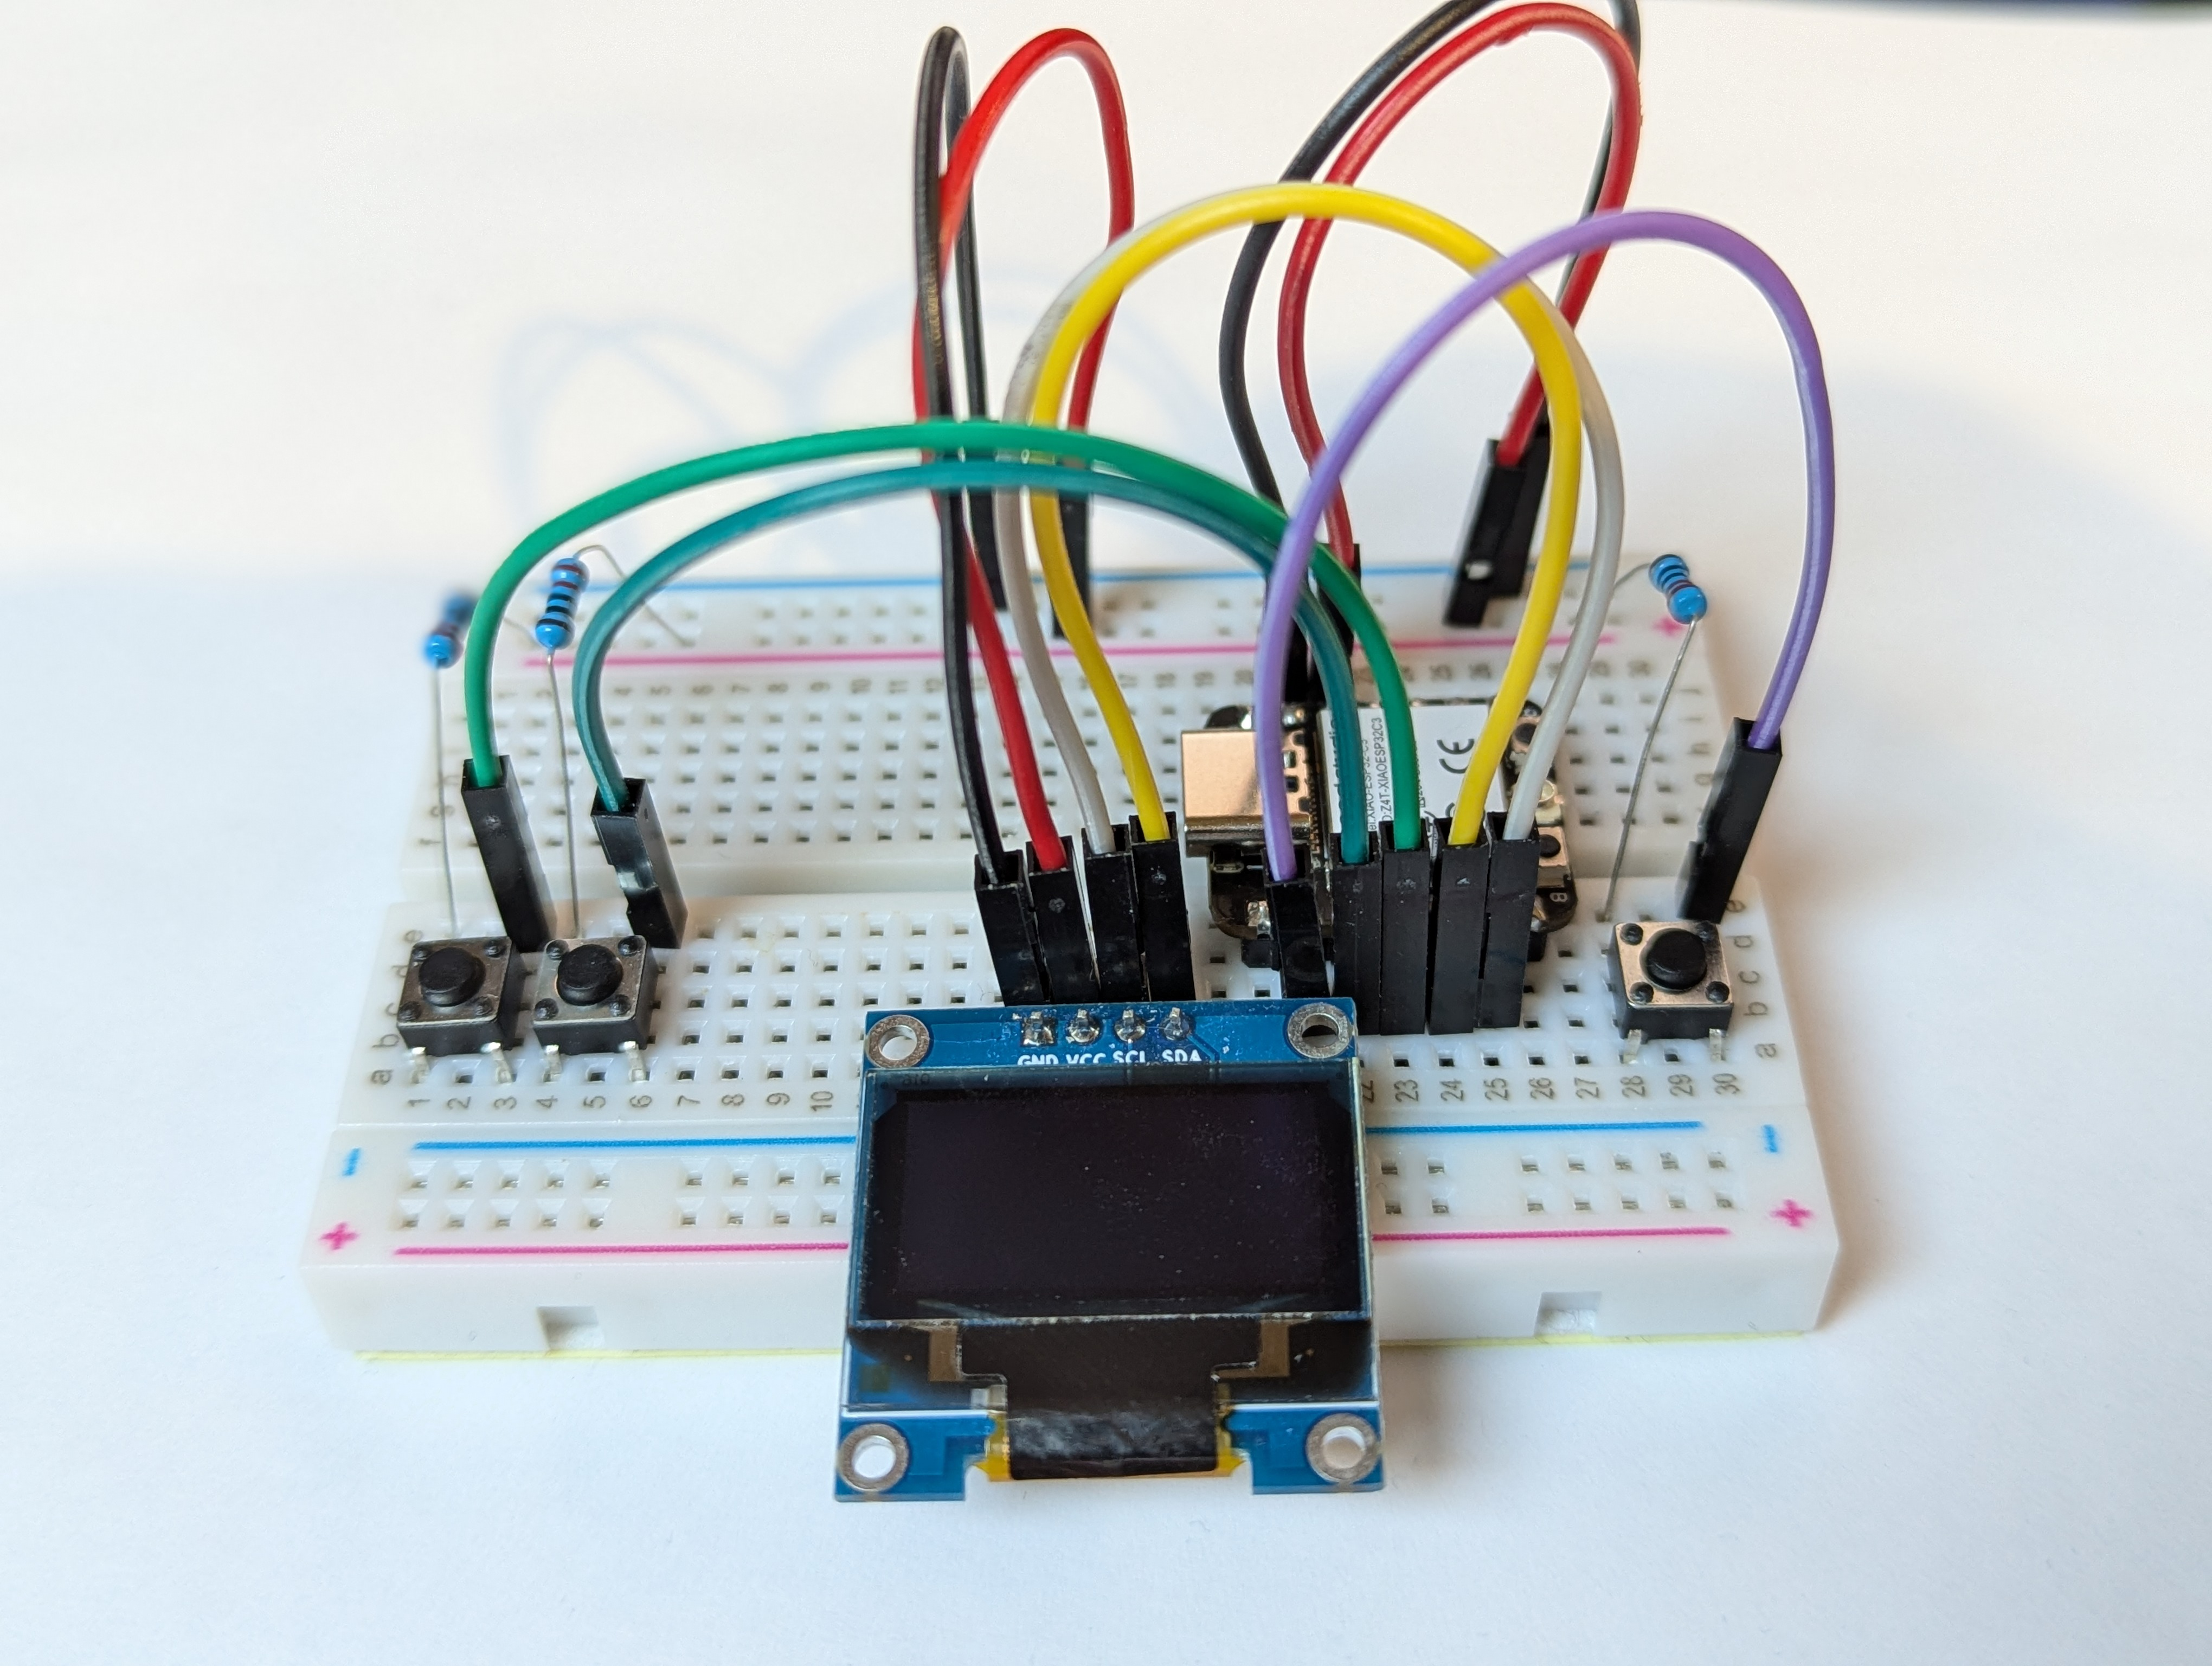
\includegraphics[width=.6\linewidth]{project_5/all_connected.jpg}
    \caption{All components and wires are now installed}
\end{figure}

\subsection{Programming the microcontroller}
Once all of the wiring is correct, connect the USB cable to the microcontroller and load the IDE to
access it. Refer back to Chapter \ref{ide} for instructions.

Click on the file named "project\_5\_game.py". This will load the code in the editor for this section. Read through the comments
and the code to get a sense for how it works. Once you are ready, you can click the blue play button in the upper left of the window
to start the game.

You can move your ship back and forth by pressing the buttons on the left. You can fire your ship's weapon by pressing the
button on the right. Once you have destroyed all of the enemy ships, a "You Win!" screen will be shown and the game will freeze.
If you want to start again, press the red stop button in the editor and then the blue play button again.

\subsection{Examining the code}

This project has the most code of any so far. The code can be broken down into several sections:
\begin{itemize}
    \item The \textbf{Missle} class
    \item The \textbf{Enemy} class
    \item The \textbf{Ship} class
    \item The \textbf{game\_loop()} function and a few helper functions (each called \textbf{update\_<x>()})
    \item A \textbf{main()} function at the bottom to get everything setup and started
\end{itemize}

Let's look at each of these below

\subsubsection{The Missle class}
\begin{lstlisting}[language=Python,caption=The Missle class]
class Missle:
"""Keeps track of an on-screen missle"""

def __init__(self, x, y):
    """Save our starting state"""
    self.x = x
    self.y = y
    self.active = True

def move(self):
    """If we move above the top of the screen, mark
    ourselves as not active. The game loop should
    cleanup any non-active missles.
    """

    global score, high_score

    self.y -= 5
    if self.y < 0:
        self.active = False

    # have we destroyed any enemies?
    for enemy in enemies:
        hitbox = enemy.hitbox
        if not hitbox[0] <= self.x <= hitbox[0] + hitbox[2]:
            continue
        if not hitbox[1] <= self.y <= hitbox[1] + hitbox[3]:
            continue
        enemy.active = False
        self.active = False
        score += 10

def draw(self):
    """Draw ourselves at our current posistion"""
    for y_offset in range(5):
        oled.pixel(self.x, self.y - y_offset, 1)
\end{lstlisting}

This class had 3 methods: an \textbf{\_\_init\_\_()} function that sets the initial state of the object,
a \textbf{move()} function that is called for each frame the missle is on screen, and a \textbf{draw()}
function which is called to tell the OLED how to display this missle.

In the \textbf{move()} function, the missle sets its position on the Y-axis upwards by 5 pixels. It then decides
if it is now higher than the top of the screen and if so, marks itself as inactive. Then it checks if it
has collided with any of the enemies that are still on the screen. If it has, it marks the enemy and
itself as destroyed and increments the player's score by 10 points.

The \textbf{draw()} function is pretty simple. It just draws a vertical line by placing 5 pixels on top of each
other, starting from the missle's current x and y coordinates.

\subsubsection{The Enemy class}
\begin{lstlisting}[language=Python,caption=The Enemy class]
class Enemy:
def __init__(self, x, y):
    self.x = x
    self.y = y
    self.active = True
    self.sprites =  [space_invaders_sprites.ENEMY_SPRITE1, space_invaders_sprites.ENEMY_SPRITE2]
    self.current_sprite = 0
    self.sprite_changed = time.ticks_ms()

@property
def hitbox(self):
    return (self.x, self.y, 16, 8)

def move(self):
    pass

def draw(self):
    now = time.ticks_ms()
    if now - self.sprite_changed > 1000:
        self.current_sprite += 1
        self.current_sprite %= len(self.sprites)
        self.sprite_changed = now
    oled.blit(self.sprites[self.current_sprite], self.x, self.y)
\end{lstlisting}

This class had 3 methods and one special method called a property. The \textbf{\_\_init\_\_()} function sets the
initial state of the object, the \textbf{move()} function that is called for each frame the enemy is on screen,
the \textbf{draw()} function is called to tell the OLED how to display this enemy. There is also a \textbf{hitbox}
property defined.

In the \textbf{\_\_init\_\_()} method, it sets some basic properties and then loads the sprite data from the external
space\_invaders\_sprites.py file. Each sprite is just an array of data that describes which pixels should be drawn
as white and which will be black. If you squint at it, you can see the shape of the enemy in the array.

The \textbf{hitbox} method is a special kind of method. It is decorated with \textbf{@property} which tells Python
to call the method and return the computed value when the property is accessed. This allows the code to dynamically
change the hitbox of the enemy if it is repositioned.

The \textbf{move()} method currently does nothing which means the enemies cannot move around the screen

The \textbf{draw()} method tells the OLED how to draw the enemy. It uses a function of the OLED library called \textbf{blit()}
which takes in the sprite data that was defined earlier and draws it to the screen in one efficient operation. This is a
much faster way that having to draw out each pixel in a loop.

\subsubsection{The Ship class}
\begin{lstlisting}[language=Python,caption=The Ship class]
class Ship:
"""Keep track of the player's ship"""

def __init__(self, x, y):
    """Save our initial state"""
    self.x = x
    self.y = y
    self.last_fired = time.ticks_ms()

def move(self):
    """Move left or right depending on which button is pressed"""

    if left_button.value() == 0:  # left pressed
        self.x -= 3
    if right_button.value() == 0:  # right pressed
        self.x += 3
    if self.x > 119:
        self.x = 119
    if self.x < 9:
        self.x = 9

def draw(self):
    """Draw the pixels of our ship"""

    oled.blit(space_invaders_sprites.SHIP_SPRITE, self.x - 8, self.y - 5)

def fire(self):
    """If the fire button is pressed and the cooldown time has
    passed, then generate a new missle object at our current position
    """

    now = time.ticks_ms()
    if fire_button.value() == 0 and now - self.last_fired > 200:
        self.last_fired = now
        missles.append(Missle(self.x, self.y - 10))
\end{lstlisting}

This class had 4 methods, the \textbf{\_\_init\_\_()} function sets the initial state of the object,
the \textbf{move()} function that is called for each frame the ship is on screen, the \textbf{draw()}
function is called to tell the OLED how to display the ship, and the \textbf{fire()} function which
checks if the fire button is pressed and creates a missle at the current ship position.

In the \textbf{move()} method, it checks if either of the left or right movement buttons are currently
pressed. If so, it moves the ship in that direction. If it detects that this ship is currently at the
edges of the screen, it doesn't move it any further.

In the \textbf{draw()} method, we use the \textbf{blit()} method mentioned previously to draw our ship's sprite to the OLED.

In the \textbf{fire()} method, we check if the fire button is currently held down. If so, it creates a new
instance of the \textbf{Missle} class and sets it's initial position to be just above the ship's current position.

\subsubsection{The game loop and helper function}
\begin{lstlisting}[language=Python,caption=The game loop and helper functions]
def update_missles():
    """Remove any non-active missles and move the rest"""

    global missles
    missles = [m for m in missles if m.active]
    for missle in missles:
        missle.move()
        missle.draw()

def update_enemies():
    """Remove any destroyed enemies and move the rest"""

    global enemies
    enemies = [e for e in enemies if e.active]
    for enemy in enemies:
        enemy.move()
        enemy.draw()

def update_score():
    global game_on
    oled.text("Score:%s" % score, 0, 0)
    if not enemies:
        oled.text("You Win!", 35, 30)
        game_on = False

def game_loop(ship):
    """Drive the main game loop"""

    oled.fill(0)
    ship.fire()
    update_missles()
    update_enemies()
    ship.move()
    ship.draw()
    update_score()
    oled.show()
\end{lstlisting}

The \textbf{game\_loop()} function is run over and over while the game is ongoing. It is responsible for
the order that all game objects are checked and redrawn. At the start of the loop it clears the entire
screen (fills all of the pixels with black). Then it checks if any new missles need to be created, updates
the existing missles, updates the enemies and the ship, and displays the current score (which also checks
if the game is over). After all objects have been updated, it tells the OLED to display everything that's
been written to it for this frame.

\subsubsection{The main function}
\begin{lstlisting}[language=Python,caption=The main function]
    def main():
    try:
        ship = Ship(64, 64)
        for y in range(12, 36, 12):
            for x in range(10, 118, 16):
                enemies.append(Enemy(x, y))
        while game_on:
            game_loop(ship)
    except KeyboardInterrupt:
        pass

main()
\end{lstlisting}

The \textbf{main()} function is pretty short, but very important. It creates instances of our ship and all
of the enemies and then runs the \textbf{game\_loop()} function over and over until the game is complete.

\section{Review}
% go over what we have accomplished (maybe go into more detail about the circuit and the pins on the microcontroller?

\section{Possible Extensions}
If you want to do some experimentation, try these:

\begin{itemize}
    \item Add some LEDs and have them light up when an enemy is hit or when the game is won.
    \item Have the enemies move around the screen. In the classic space invaders game, they moved down towards the ship as the game progressed.
\end{itemize}

\chapter{Project 6: Web}

\section{Overview}
A piece of hardware that we haven't talked about yet which is built into the ESP32-C3 microcontroller
is it's WiFi processor. We can make use of this to connect to the internet and pull in all kinds of
data or transmit data to other services! If you've ever heard the phrase "Internet of Things", this
is what they mean. Over the course of this project, you will:
\begin{itemize}
    \item Use the embedded WiFi processor to connect to the internet
    \item Make requests to free 3rd party API services to fetch live data
    \item Use the connected buttons and screen to display different sets of that data
\end{itemize}
At the end of this project, your microcontroller should run a MicroPython program that displays 3
different screens of data that you can rotate through with the buttons. Let's get started!
\begin{figure}[H]
\centering
    \includegraphics[width=.6\linewidth]{project_6/screen_connected.jpg}
    \caption{The end result should look something like this}
\end{figure}

\pagebreak

\section{Directions}

\subsection{Creating the circuit}
Using jumper cables, you will be assembling a circuit between your microcontroller, your breadboard, two
buttons and the small OLED screen included in your kit.

\subsubsection{Remove previous components}
Before beginning, remove any components from prior chapters including LEDs, buttons, and wires. You may leave the
microcontroller attached to the breadboard.

\subsubsection{Attach the microcontroller to the breadboard}
If it's not already, carefully insert the pins at the bottom of your microcontroller into the breadboard. Refer back
to \ref{pinout} for pin labels. When placing the board into the breadboard, make sure that the microcontroller is oriented such that:
\begin{itemize}
    \item The pin labeled \textbf{5V} is inserted in hole at \textbf{Column H, Row 1} of the breadboard (or \textbf{H1}, for short)
    \item The pin labeled \textbf{GPIO2} is inserted in hole \textbf{D1} of the breadboard
    \item The pin labeled \textbf{GPIO20} is inserted in hole \textbf{H7} of the breadboard
    \item the pin labeled \textbf{GPIO21} is inserted in hole \textbf{D7} of the breadboard
\end{itemize}
You may need to apply more pressure than expected to seat the microcontroller properly in the breadboard. When its over, it should look like this:
\begin{figure}[H]
    \centering
    \includegraphics[width=.6\linewidth]{common/microcontroller_seated_in_breadboard.jpg}
    \caption{So far, so good!}
\end{figure}

\subsubsection{Place the OLED Screen and Buttons on the Board}
\begin{itemize}
    \item Place the OLED screen into the breadboard such that its 4 pins connect to holes \textbf{A12}, \textbf{A13}, \textbf{A14}, and \textbf{A15}.
    \item Place a button so that one connected set of pins (refer to \ref{button_basics} for an example) is in \textbf{E21}
    and \textbf{F21} and the other set is in \textbf{E23} and \textbf{F23}.
    \item Place a resistor between \textbf{G21} and the top negative rail (the blue one).
    \item Place another button so that one connected set of pins is in \textbf{E28} and \textbf{F28}
    and the other set is in \textbf{E30} and \textbf{F30}.
    \item Finally place a resistor between \textbf{G28} and the top negative rail.
\end{itemize}

You should be left with something that looks like this:
\begin{figure}[H]
    \centering
    \includegraphics[width=.6\linewidth]{project_6/components_placed.jpg}
    \caption{All of the components except for the jumper wires are now placed.}
\end{figure}

\subsubsection{Connect the necessary jumper wires}
\begin{itemize}
    \item Using a black jumper wire, place one end of the wire into hole \textbf{J2} of the breadboard and the other
    end into any hole on the top negative rail (the blue one). This will provide the ground connection for all components.
    \item Place another black jumper wire between the top negative rail and \textbf{C12}, the GND connection of the OLED.
    \item Place a red jumper wire into hole \textbf{J3} of the breadboard and the other end into
    \textbf{C13}. This will provide \textbf{3.3} volts of power to the OLED.
    \item Place a white jumper wire between \textbf{C14} and \textbf{B6}. This will provide a clock signal to the OLED screen.
    \item Place a yellow jumper wire between \textbf{C15} and \textbf{B5}. This will provide the data to display on the OLED screen.
    \item Place a green jumper wire between \textbf{J23} and \textbf{J6}. This will provide the signal to move to the previous screen.
    \item Place a green jumper wire between \textbf{J30} and \textbf{J7}. This will provide the signal to move to the next screen.
    \item Finally, attach the antenna to the microcontroller by plugging the gold end of its wire into the socket in the bottom of
    the microcontroller's board, between the buttons.
\end{itemize}

You should be left with something that looks like this:
\begin{figure}[H]
    \centering
    \includegraphics[width=.6\linewidth]{project_6/wired_up.jpg}
    \caption{All components and wires are now installed}
\end{figure}

\subsection{Programming the microcontroller}
Once all of the wiring is correct, connect the USB cable to the microcontroller and load the IDE to
access it. Refer back to Chapter \ref{ide} for instructions.

Click on the file named "project\_6\_web.py". This will load the code in the editor for this section. Read through the comments
and the code to get a sense for how it works. You will need to edit the code and provide values for the WiFi network name
and password before it will work:

\begin{figure}[H]
    \centering
    \includegraphics[width=.6\linewidth]{project_6/enter_wifi_credentials.png}
    \caption{If you are doing this during the workshop at NetApp, these will be given to you. If you are at home, use the credentials for your house.}
\end{figure}

Once you are ready, you can click the blue play button in the upper left of the window
to start the program.

You can press the left and right buttons to rotate through the different views on the screen. Note that it takes
a few seconds for the microcontroller to load and parse the data from each API. This can sometimes lead to
buggy behavior when pressing the buttons quickly.

\subsection{Examining the code}

This project's code shows a few new concepts:
\begin{itemize}
    \item Configuring the microcontroller's WiFi hardware and connecting to a network
    \item Making requests to a web-based API
    \item Parsing the results of the API and displaying them on our screen
\end{itemize}

Let's take each of these and examine them closer

\subsubsection{Connecting to WiFi}
\begin{lstlisting}[language=Python,caption=WiFi Code]
import network

# You must provide values for these that match the WiFi network you would like to
# connect to.
NETWORK_NAME = ""
NETWORK_PASSWORD = ""

def connect_to_wifi():
    if not NETWORK_NAME or not NETWORK_PASSWORD:
        print("Don't forget to fill in the WiFi details at the top of the script!")
        return False

    print(f"Connecting to {NETWORK_NAME}...")
    OLED.text("Connecting...", 12, 25)
    OLED.show()

    interface = network.WLAN(network.STA_IF)
    interface.active(True)
    interface.connect(NETWORK_NAME, NETWORK_PASSWORD)
    tries = 10
    while tries > 0:
        if not interface.isconnected():
            tries -= 1
            time.sleep(1)
        else:
            print(f"Connected to {NETWORK_NAME} successfully")
            break
    else:
        print(f"Failed to connect to {NETWORK_NAME}. Is the password correct?")
        return False

    return True
\end{lstlisting}

In the listing above, we see just the code that is responsible for setting up the WiFi hardware and connecting
to the network. First we import the network module. This is part of the standard library for MicroPython.
In the \textbf{connect\_to\_wifi()} function, we make sure the network name and password are set. Then
we print out a status message to let the user know that something is happening. Then we get the \textbf{interface}
object by asking the \textbf{network} library to give us a handle to the microcontroller's WiFi chip. We mark
the \textbf{interface} as active and tell it to connect with the credentials the user gave us.

It takes a little time to connect to the WiFi router, so we have a loop to wait until that happens. If we
get connected, then we will exit the function returning \textbf{True}. If something prevents us from conencting,
for example a mistyped password, then we will print a message to let the user know and return \textbf{False}.

\subsubsection{Talking to an API}
\begin{lstlisting}[language=Python,caption=Making Web Requests]
def draw_date_and_time():
    # Use the timeapi.io site to fetch the current time
    # using the IP address of our microcontroller
    # https://timeapi.io/swagger/index.html
    response = requests.get(f"https://timeapi.io/api/time/current/ip?ipAddress={IP_ADDRESS}")
    date_time = response.json()
    OLED.fill(0)
    OLED.text(f"{date_time['hour']:02d}:{date_time['minute']:02d}:{date_time['seconds']:02d}", 30, 5)
    OLED.text(f"{date_time['dayOfWeek']}", 35, 15)
    OLED.text(f"{date_time['date']}", 20, 25)
\end{lstlisting}

In the above code, we make use of our new network connection by making an HTTP GET request to the \url{https://timeapi.io/}
site. This site provides a JSON-based RESTful API that anyone can use. The URL that we make the request to is
asking for the current time at the IP address that we were assigned when we connected to WiFi. If we made this request
in our browser, the response would look something like this:

\begin{figure}[H]
    \centering
    \includegraphics[width=.6\linewidth]{project_6/api_response.png}
    \caption{An example response from the timeapi.io site}
\end{figure}

This format is called JSON. It is a way of expressing groups of data that many programming languages can
understand. It is one of the most common formats for web-based APIs. In our code, we use the \textbf{response.json()}
function to parse this response into a Python dictionary object. We can then access the fields of the response in
our code and print them out on our screen.

\section{Review}
This chapter is an example of how you might create an Internet of Things device using a microcontroller and
some Python code. While our example is small, you could imagine that instead of our small screen, we are
displaying this on a large touch screen, perhaps one acting as the bathroom mirror. Then when you were getting
ready each day, the things most relevant to you would be readily visible.

\section{Possible Extensions}
If you want to do some experimentation, try these:

\begin{itemize}
    \item Change the code to auto-cycle between the screens every X seconds even without a button press
    \item Find another web-based API that is free and accessible and display information from it on a 4th screen
\end{itemize}


\chapter{Project 7: Chat}
% chapter contents


\appendix
\chapter{Electronics Essentials}
% chapter contents
\chapter{Python Primer}
If you're new to Python, this section will give you a few things you should know
in order to better understand the projects in this guide. This is by no means a
complete or comprehensive look at the Python language. For that, we recommend looking
at the official Python site and reading through the \href{https://docs.python.org/3/tutorial/}{tutorial}
there.

\begin{tcolorbox}
    Note: for the projects being used here, we are using an implementation of
    Python known as \href{https://micropython.org/}{MicroPython}. This version
    is meant to run on microcontrollers with limited resources. It
    also has built into it libraries for dealing with hardware devices that are
    not part of the standard CPython distribution. Therefore, not all Python examples
    you find online will run on your microcontroller and not all projects for a
    microcontroller can be run on your computer. But a lot of the code can be shared
    so the lessons you learn here can apply to other Python projects.
\end{tcolorbox}

Here is a sample of a small Python script. We will disect and explain what each
section does below:

\begin{lstlisting}[language=Python,caption=An example Python script]
def show(message, repeat=1):
    """This function prints the given message to the
    console as smany times as specified in the
    srepeat parameter.
    """

    for iteration in range(0, repeat):
        print(iteration, message)

name = input("What is your name: ")
show(name)
show(name, repeat=3)
\end{lstlisting}

On line 1, we are defining a function named show. This function accepts two parameters,
message and repeat. The message parameter is required and the repeat parameter
is optional with a default value of 1.

Lines 2 through 5 comprise the docstring for the function. This information is meant
for programmers to read and explains what the function does. It does not affect how
the function works.

Line 7 starts a loop. The loop will repeat the statements in the loop body until
a condition is met. In this case, it will loop until it has performed the operation
for each repeat.

Line 8 is the body of the loop. This statement will print the message that the user
passed in to the console along with the iteration number of the loop.

Line 10 prompts the user for their name and saves the result in a variable called
name.

Line 11 calls our show function which will print the user's name once (the default).

Line 12 calls our show function again, this time saying that we want to repeat the
loop of printing the name twice.\newline

Running the program, we will see output like this:
\begin{verbatim}
$ python program.py
What is your name: Emily
0 Emily
0 Emily
1 Emily
2 Emily
$
\end{verbatim}

Another feature that you'll see used often in Python are classes. Classes are a
convienent way to model something in your program that holds state and implements
functionality. For example, let's say that we are writing a game about racing go-
karts. We need to allow each player to have their own kart and keep track of how
fast it is going, which way they are turning, and allow the kart to speed up and
slow down. Here is a small class that will help us do that:

\begin{lstlisting}[language=Python,caption=An example of a Python class]
class Kart:
    MAXIMUM_SPEED = 100

    def __init__(self):
        """The kart starts motionless at the beginning"""
        self._speed = 0
        self._direction = 0
        self._acceleration = 0

    def brake(self):
        """This is called when the user presses the brake button"""
        self._acceleration = -5

    def accelerate(self):
        """This is called when the user presses the accelerator button"""
        self._acceleration = 5

    def steer(self, direction):
        """This is called when the user presses left or right"""
        self._direction = direction

    def update(self, ticks):
        """Update will be called by our game engine and will be
        provided the number of ticks since it was last called.
        """

        self._speed += self._acceleration * ticks

        # limit our speed so that we don't go faster than our
        # kart is allowed to, or slower than 0
        if self._speed > Kart.MAXIMUM_SPEED:
            self._speed = Kart.MAXIMUM_SPEED
        if self._speed < 0:
            self._speed = 0
\end{lstlisting}

Looking at this class, there are 5 methods. The first one (on line 4) is a special
method that is called by the Python interpreter whenever a new Kart is created. It
will initialize some variables for this particular Kart object.

You may have noticed that the first method takes a parameter called "self". This
is the first parameter of all methods in a class in Python. It is automatically passed
by the interpreter and is a reference to the current object. It lets us access the
variables that belong to the class, like those we defined in the \_\_init\_\_ method.

Speaking of the variables in the \_\_init\_\_ method. Notice how we named them all with
an underscore? This is a convention in Python that says they are private to our class
and that code written outside of the class shouldn't access them directly. That means
that our class should provide ways to modify or read these variables via other methods.

The second method starts on line 10. This is called when the player presses the
brake button on their controller and will set our Kart's acceleration to a negative
value so that we start to slow down. It modifies the private \_acceleration member of
the class.

The third starts on line 14. It is the opposite of braking and will start speeding
our Kart up when the user presses the accelerator. It aslo modifies the private
\_acceleration member of the class.

The fourth method, line 18, is again something to deal with user input. This time
we can see that it takes a second parameter, direction. If the user presses left on
their controller, then we can expect left to be passed here. The same for right. We
will modify the private \_direction member here.

Finally, we have a fifth method starting on line 22. This method is called by our
game engine and uses the class members to determine what happens to the Kart throughout
the game. That is, it is asking the Kart to update itself at a certain moment in time
(usually once per frame) so that next time it draws it to the screen, it will be
in the updated location.

Notice in the last method, we are accessing not only our own variables, \_speed, and
\_acceleration, but we are also reading a class variable, Kart.MAXIMUM\_SPEED. Unlike
our member variables, a class variable is the same for all instances of a class. It
is useful here to keep the game fair so that all Karts have the same limitation on
their speed.

\end{document}
